\chapter[Revisão de literatura ]{Revisão de literatura}

Nesta seção são abordados conceitos fundamentais para a compreensão deste trabalho, assim como tendências atuais da literatura em relação ao tema estudado.

\section{O problema da dimensionalidade}

Sistemas que se utilizam de aprendizado de máquina apresentam respostas baseados nos dados de entrada que lhe são apresentados. Dessa maneira, a determinação de que variáveis são relevantes para o sistema é uma etapa fundamental de seu processo de desenvolvimento.

A inclusão de variáveis irrelevantes resulta no aumento da complexidade do modelo, o tornando mais suscetível ao \textit{overfitting} e menos interpretável \cite[p. 204]{intro_stat_learn}. Além disso, um número elevado de variáveis de entrada resulta em um efeito conhecido como a maldição da dimensionalidade (\textit{curse of dimensionality}), onde o aumento do número de dimensões (quantidade de variáveis), implica no aumento exponencial do número de amostras necessárias para representar o espaço de variáveis \cite[p. 34]{bishop_2006}.

\begin{figure}[H]
    \centering
    \caption{Crescimento do espaço de variáveis em virtude do aumento das dimensões.}
    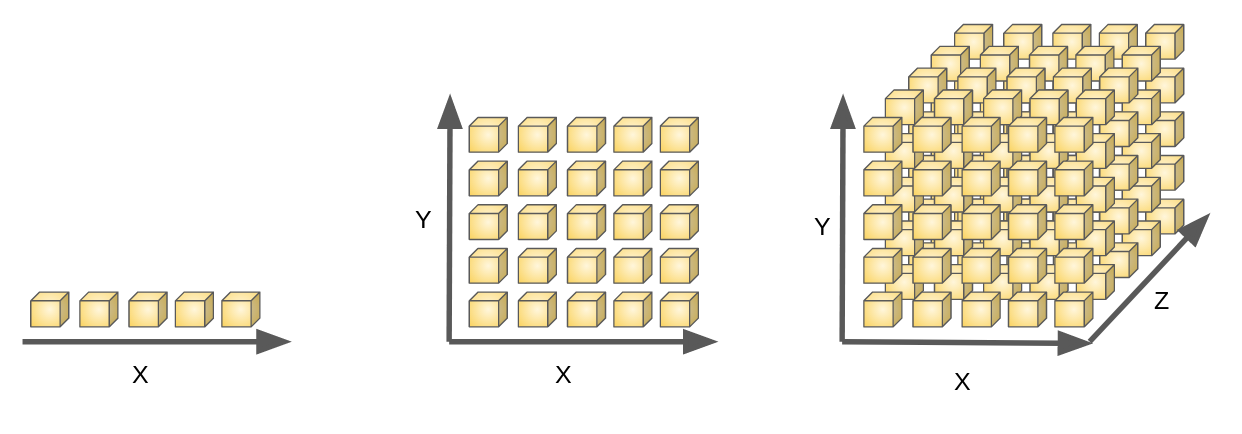
\includegraphics[width=0.8\textwidth]{imgs/rev/dimensionalty_grown.png}
    \legend{Fonte: The Curse of Dimensionality \cite{dim_grown}}
    \label{fig:dim_grown}
\end{figure}

\begin{figure}[H]
    \centering
    \caption{Performance em relação ao número de dimenções e amostras.}
    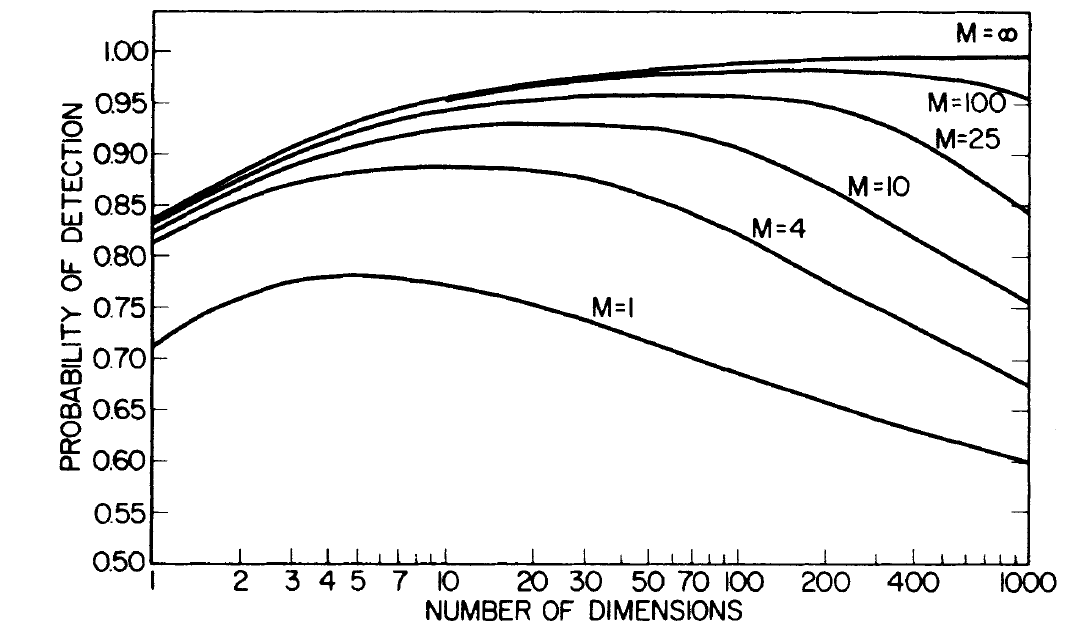
\includegraphics[width=0.5\textwidth]{imgs/rev/dim_performance}
    \legend{Fonte: A Problem of Dimensionality: A Simple Example \cite{art:prob_dim}}
    \label{fig:dim_perf}
\end{figure}


É desejável então que se utilize o menor número possível de variáveis de entrada que permitam ao modelo produzir a resposta correta. Uma maneira de realizar essa redução de dimensionalidade é selecionar um subconjunto das variáveis disponíveis, descartando aquelas que apresentarem pouca ou nenhuma relevância para o problema \cite[p. 204]{intro_stat_learn}.


\section{Regressão Linear}

Os modelos de regressão linear constituem uma classe de modelos que utilizam funções lineares com parâmetros ajustáveis. O exemplo mais simples dessa classe é a função que realiza a combinação linear das entradas com os parâmetros ajustados para gerar uma predição (eq. \ref{eq:lin_expandida}).

\begin{equation}
    \hat{y} = w_0 + w_1*x_1+ ... + w_Dx_D = \sum_{i = 0}^{D} w_i\phi(x_i) = \phi(X)W
    \label{eq:lin_expandida}
\end{equation}

Onde $D$ corresponde ao número de dimensões da variável de entrada, $x_0 = 1$ e $\phi(x_i) = x_i$.

Modelos mais complexos e de maior aplicabilidade podem ser obtidos ao se considerar um conjunto fixo de transformações não-lineares ($\phi_n(x)$) ao invés das variáveis originais, ou em conjunto com elas. Esses modelos são lineares em relação as suas variáveis independentes, porém são não-lineares em relação as variáveis de entrada \cite{bishop_2006}.

\subsection{Treinamento de modelos lineares}

O treinamento de modelos lineares consiste em encontrar o vetor de parâmetros $W$ que maximize a similaridade entre o modelo e sistema modelado. Esse treinamento é normalmente realizado minimizando-se o somatório dos erros quadráticos (eq. \ref{eq:sq_error}) em função do vetor $W$.

% \begin{align}
% \begin{split}
%       E_{sq}(W) {}&= \frac{1}{2} \sum_{n = 1}^{N}\left(y_n-\hat{y}_n\right)^2 = \frac{1}{2} \sum_{n = 1}^{N} \left(y_n-\phi(X_n)W\right)^2
%     \label{eq:sq_error}  
% \end{split}\\
% \begin{split}
%     \pdv{E_{sq}(W)}{W} {}&= \sum_{n = 1}^{N} \phi(X_n)^T\left(\phi(X_n)W - y_n\right)
%     \label{eq:min_sq_error}
% \end{split}
% \end{align}

\begin{equation}
\begin{split}
      E_{sq}(W) {}&= \frac{1}{2} \sum_{n = 1}^{N}\left(y_n-\hat{y}_n\right)^2 \\
      &= \frac{1}{2} (Y-\hat{Y})^T(Y-\hat{Y})\\
      &= \frac{1}{2} \left( Y^TY - 2 \hat{Y}^TY + \hat{Y}^T\hat{Y} \right)\\
      &= \frac{1}{2} \left( Y^TY - 2 W^T\phi(X)^TY + \sum_{n = 1}^{N}\left(\phi(X_n)W \right)^2 \right)
    \label{eq:sq_error}  
\end{split}
\end{equation}

\begin{equation}\begin{split}
    \pdv{E_{sq}(W)}{W} {}&= \frac{1}{2} \left( 0 - 2 \phi(X)^TY + 2\sum_{n = 1}^{N}\left(\phi(X_n)^T\phi(X_n) \right)W  \right) \\
    &= - \phi(X)^TY + \phi(X)^T\phi(X) W
    \label{eq:min_sq_error}
\end{split}\end{equation}

Igualando-se a eq. \ref{eq:min_sq_error} a zero e isolando o vetor $W$, obtém-se a eq. \ref{eq:lsnormal}, conhecida como a equação normal para o problema dos mínimos quadrados.

\begin{equation}\begin{split}
    \phi(X)^T\phi(X) W &= \phi(X)^TY \\
    W &= (\phi(X)^T\phi(X))^{-1}\phi(X)^TY \\
    W &=\phi(X)^+ Y
    \label{eq:lsnormal}
\end{split}\end{equation}

O termo $(\phi(X)^T\phi(X))$ pode se aproximar de uma matriz singular se muitas das variáveis envolvidas forem linearmente dependentes, resultando assim em dificuldades para o cálculo numérico dos valores e possivelmente em um vetor de parâmetros de alta magnitude. Um termo de regularização na eq. \ref{eq:sq_error} resolve esse problema, garantindo que a nova matriz não é singular. A dedução da equação normal com termo de regularização é análoga à apresentada e o resulta na eq. \ref{eq:lsnormal_reg}.

\begin{equation}\begin{split}
    W &= (\lambda I + \phi(X)^T\phi(X))^{-1}\phi(X)^TY = A^{-1}\phi(X)_{[i]}^TY
    \label{eq:lsnormal_reg}
\end{split}\end{equation}

A adição do termo de regularização tem ainda o efeito de limitar a complexidade efetiva do modelo, reduzindo o \textit{overfitting} e possibilitando a utilização de conjuntos de dados menores \cite{bishop_2006}.

\section{Validação Cruzada}

A validação cruzada (\textit{cross-validation}) é um conjunto de metodologias de treinamento e validação que, de maneira simples e efetiva, permitem a estimativa do erro de generalização do modelo.

No método \textit{k-fold} de validação cruzada, os dados de treinamento são divididos em k conjuntos aleatórios de tamanhos aproximadamente iguais. Realizada essa divisão, a cada iteração do treinamento, os parâmetros do modelo são determinados utilizando k-1 conjuntos e sua performance é avaliada no conjunto restante. O processo se repete até que todos os k conjuntos tenham sido utilizados para avaliação e a média das performances observadas fornecem uma estimativa da performance de generalização do modelo \cite{overfitting_crossval}.

\begin{figure}[H]
    \centering
    \caption{Validação cruzada: \textit{5-fold}.}
    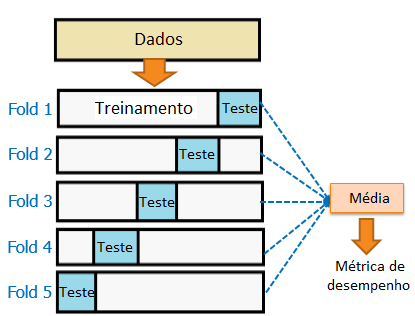
\includegraphics[width=0.7\textwidth]{imgs/rev/cross_validation}
    \legend{Fonte: Different types of Validations in Machine Learning (Cross Validation) \cite{cross_val}}
    \label{fig:dim_perf}
\end{figure}

Um caso especial do método descrito é o \textit{leave-one-out cross-validation} (LOOCV), onde k é igual ao total de 
amostras disponíveis (N), ou seja, o treinamento é realizado N vezes com N-1 amostras, e validado na amostra excluída.
 Tal abordagem apesar de apresentar, em geral, um custo computacional elevado, resulta em um modelo com menor 
 variabilidade e viés para modelos de regressão linear \cite{burman}, produzindo assim resultados com melhor 
 performance e menos \textit{overfitting}.

\subsection{ \textit{Leave-one-out Cross-validation} e Regressão Linear}

Especificamente para o caso do preditor linear, é possível determinar o resultado do LOOCV sem a necessidade de se 
calcular N preditores, tornando essa uma estratégia interessante para determinar a capacidade de generalização de 
um modelo linear. A seguir uma dedução adaptada de \cite[p. 268]{lin_reg_analysis} é apresentada.

O erro de LOOCV corresponde a média dos erros quadráticos de cada estimador obtido excluindo-se uma amostra. 

\begin{equation}
    LOOCV = \dfrac{1}{N} \sum_{i=1}^{N}e^2_{[i]}
    \label{eq:cv_error}
\end{equation}
\begin{equation}
    e_{[i]} = y_i - \hat{y}_{[i]} = y_i - x_iW_{[i]} 
    \label{eq:ith_error}
\end{equation}
Onde o $i$ indexa a amostra excluída no treinamento, $\hat{y}_{[i]}$ corresponde à saída do preditor calculado sem a
amostra $(x_i,y_i)$ e $W_{[i]}$ os parâmetros desse preditor.

Pode-se definir o vetor de parâmetros $W_{[i]}$ conforme a eq. \ref{eq:wi}.
\begin{equation}
    W_{[i]} = A_{[i]}^{-1}\phi(X)_{[i]}^TY_{[i]}
    \label{eq:wi}
\end{equation} 

É possivel perceber as seguintes igualdades:
\smallskip\noindent
\begin{equation}
    \begin{split}
        A_{[i]} &= \lambda I + \phi(X)_{[i]}^T\phi(X)_{[i]} \\
                &= \lambda I + \phi(X)^T\phi(X) - x_i^Tx_i \\
                &= A - x_i^Tx_i    
    \end{split}
    \label{eq:ai_identity}
\end{equation} 

\begin{equation}
    \phi(X)_{[i]}^TY_{[i]} = \phi(X)^TY - x_i^Ty_i
    \label{eq:X_iY_i_identity}
\end{equation} 

Aplicando a formula de Sherman–Morrison à eq. \ref{eq:ai_identity}, temos:
\smallskip\noindent
\begin{equation}
    \begin{split}        
       h_i &= x_iA^{-1}x_i^T \\
       A_{[i]}^{-1} &= A^{-1} + \dfrac{A^{-1}x_ix_i^TA^{-1}}{1-h_i}
    \end{split}
    \label{eq:sherman}
\end{equation}

Substituindo as eq. \ref{eq:X_iY_i_identity} e \ref{eq:sherman} na eq. \ref{eq:wi}.
\smallskip\noindent
\begin{equation}
    \begin{split}
        W_{[i]} &= \left(A^{-1} + \dfrac{A^{-1}x_i^Tx_iA^{-1}}{1-h_i}\right) \left(\phi(X)^TY - x_i^Ty_i\right)\\
                &= W - A^{-1}x_i^Ty_i + \dfrac{A^{-1}x_i^Tx_iW}{1-h_i} - \dfrac{A^{-1}x_i^Tx_iA^{-1}x_i^Ty_i}{1-h_i} \\
                &= W - \dfrac{A^{-1}x_i^T}{1-h_i}\left(  y_i(1-h_i)-x_iW  + h_iy_i \right)  \\
                &= W - \dfrac{A^{-1}x_i^T}{1-h_i}\left(  y_i-\hat{y}_i \right)  \\
    \end{split}
    \label{eq:wi_expandido}
\end{equation}

Substituindo as eq. \ref{eq:wi_expandido} na eq. \ref{eq:ith_error}.
\smallskip\noindent
\begin{equation}
    \begin{split}
        e_{[i]} &= y_i - x_iW_{[i]} \\
                &= y_i - x_i\left( W - \dfrac{A^{-1}x_i^T}{1-h_i}\left(  y_i-\hat{y}_i \right) \right) \\
                &= y_i - \hat{y}_i + \dfrac{h_i}{1-h_i}\left(  y_i-\hat{y}_i \right) \\
                &= \dfrac{y_i- \hat{y}_i}{1-h_i}
    \end{split}    
    \label{eq:ith_error_expandido}
\end{equation}

Seja $P$ a matriz de projeção \cite[p. 303]{applied_matrix_algebra} do preditor (também conhecida como matriz chapéu
 \cite[p. 266]{lin_reg_analysis}) e a matriz $R$ definida conforme a eq. \ref{eq:proj_res_matrix}
\smallskip\noindent
\begin{equation}
    \begin{split}
        \hat{Y} &= PY \implies P = XA^{-1}X^T \\
        RY &= Y - \hat{Y} \implies R = I - P = I - XA^{-1}X^T
    \end{split}    
    \label{eq:proj_res_matrix}
\end{equation}

Para cada índice $i$, o numerador da eq. \ref{eq:ith_error_expandido} corresponde a linha de mesmo índice da matriz $RY$. 
Além disso o denominador da equação corresponde ao elemento da diagonal da matriz $R$ de mesmo índice. 
A partir dessas observações, pode-se agrupar todos os valores de $e_{[i]}$ na forma da matriz $E_{LOOCV}$, conforme a equação \ref{eq:e_cv}.
\smallskip\noindent
\begin{equation}
    \begin{split}
        E_{LOOCV} = diag(R)^{-1}RY
    \end{split}    
    \label{eq:e_cv}
\end{equation}

Dessa forma a eq. \ref{eq:cv_error} pode ser reescrita conforme eq. \ref{eq:LOOCV_error}.

\begin{equation}
    \begin{split}
        LOOCV   &= \dfrac{1}{N} \sum_{i=1}^{N}e^2_{[i]} \\
                &= \dfrac{1}{N} E_{LOOCV}^2 \\
                &= \dfrac{1}{N}E_{LOOCV}^TE_{LOOCV} \\
                &= \dfrac{1}{N} Y^TR\ diag(R)^{-2}RY \\
    \end{split}
    \label{eq:LOOCV_error}
\end{equation}